\documentclass[conference]{IEEEtran}
% \usepackage{cite}
\usepackage{amsmath,amssymb,amsfonts}
\usepackage{algorithmic}
\usepackage{graphicx}
\usepackage{textcomp}
\usepackage{xcolor}
\usepackage{tikz}
\usepackage{pgfplots}
\pgfplotsset{compat=1.18}
\usetikzlibrary{shapes.geometric, arrows.meta, positioning, fit, calc, shadows}

\def\BibTeX{{\rm B\kern-.05em{\sc i\kern-.025em b}\kern-.08em
    T\kern-.1667em\lower.7ex\hbox{E}\kern-.125emX}}

\begin{document}

\title{Vehicle Speed Estimation from Single-Channel Audio using Amplitude-Preserving SE-ResNet\\
}

\author{\IEEEauthorblockN{Anonymous Authors} \\
% Author block will go here
}

\maketitle

\begin{abstract}
% We will write this after ablation.
\end{abstract}

\begin{IEEEkeywords}
Intelligent Transportation Systems, Acoustic Sensing, Deep Learning, Squeeze-and-Excitation, Vehicle Speed Estimation
\end{IEEEkeywords}

\section{Introduction}
\label{sec:introduction}
\IEEEPARstart{P}{recise} speed quantification is a critical component of Intelligent Transportation Systems (ITS), enabling applications from traffic flow analysis to automated enforcement. While traditional modalities such as radar, LiDAR, and optical cameras are effective, they are often hindered by high deployment costs, line-of-sight dependencies, and privacy issues related to identifying markers like license plates. Passive acoustic sensing represents a promising alternative, utilizing the pervasive sound generated by moving vehicles. This acoustic footprint—arising from engine combustion, tire friction, and aerodynamic turbulence—encodes velocity information primarily through Doppler shift patterns.

Early research in this domain largely depended on parametric models with manually tuned coefficients, typically validated in controlled settings with limited vehicle variety \cite{ref1, ref2}. More recent works have explored 1D convolutional neural networks on raw waveforms \cite{ref4} or physics-inspired features with support vector regression \cite{ref5, ref13}. The current state-of-the-art \cite{ref10} achieves high accuracy but relies on a fusion of audio and visual data, which reintroduces hardware complexity and privacy concerns.

\subsection{Problem Statement and Research Gap}
Despite growing interest in deep learning for acoustic speed estimation, a systematic evaluation of modern \textit{attention-augmented} 2D convolutional architectures remains absent. Existing 2D-CNN studies have mostly used plain ResNets or shallow networks without explicit channel-wise recalibration \cite{ref9}. Meanwhile, transformer-based models, although powerful, tend to overfit on small-to-medium datasets like VS13 (only 400 clips) due to their low inductive bias. On the other hand, multimodal systems \cite{ref10} achieve superior accuracy but require synchronized cameras and microphones, increasing cost and limiting deployment in privacy-sensitive zones. Hence, there is a clear need for a purely acoustic, single-sensor solution that can compete with hybrid systems while preserving the low-cost and non-intrusive nature of passive sensing.

\subsection{Motivation}
The Squeeze-and-Excitation (SE) mechanism \cite{ref12} has proven effective in image classification by adaptively recalibrating channel-wise feature responses. When applied to Mel spectrograms, SE blocks can emphasize frequency bands that carry Doppler shift information—directly correlated with vehicle speed—while suppressing stationary noise. This built-in attention is particularly suited to audio regression tasks, where relevant spectral patterns vary with time and speed. Moreover, ensemble learning through cross-validation can reduce prediction variance and provide a realistic upper bound on performance. Therefore, we are motivated to combine SE-ResNet with a well-designed ensemble strategy to push the limit of single-modality acoustic speed estimation.

\subsection{Contributions}
The primary contributions of this work are summarized as follows:
\begin{itemize}
    \item \textbf{Leakage-Free Nested Cross-Validation Protocol:} We establish a rigorous nested cross-validation (Nested CV) methodology tailored to compact acoustic datasets (VS13, 400 samples), strictly isolating outer generalization evaluation from inner hyperparameter selection to eliminate optimism bias.
    \item \textbf{Asynchronous Dual-GPU Optimization Infrastructure:} We design a decentralized, non-blocking Bayesian hyperparameter optimization engine utilizing Optuna \cite{ref11} with a Tree-structured Parzen Estimator (TPE) and SQLite locking, executing across dual NVIDIA T4 GPUs without inter-process distributed communication overhead.
    \item \textbf{Tripartite Component Ablation:} We perform systematic ablation studies that independently isolate: (i) the Squeeze-and-Excitation attention mechanism across reduction ratios $r \in \{8, 16, 32\}$, (ii) hierarchical network depth ($2, 3,$ and $4$ residual stages), and (iii) stochastic environmental acoustic augmentations.
    \item \textbf{Statistical Error Profiling and Inferential Analysis:} We conduct a formal One-Way ANOVA test across 13 vehicle classes and analyze residual distributions across low, medium, and high velocity regimes ($30\text{--}105$~km/h), confirming error homoscedasticity and quantifying the acoustic factors driving class variance.
    \item \textbf{State-of-the-Art Single-Modality Accuracy:} The proposed ensembled SE-ResNet achieves an RMSE of \textbf{7.29~km/h}, outperforming all existing single-sensor acoustic methods and closing the gap to complex audio-visual fusion systems to within $0.75$~km/h.
    \item \textbf{Open Science:} All code, model weights, and hyperparameter optimization study logs are made publicly available to ensure complete reproducibility.
\end{itemize}

\subsection{Paper Organization}
The remainder of this paper is structured as follows. Section II reviews related work on acoustic vehicle speed estimation, highlighting benchmark datasets and the research gap. Section III describes the VS13 dataset, data preprocessing, the SE-ResNet architecture, the nested cross-validation scheme, and the asynchronous dual-GPU optimization setup. Section IV presents empirical results, including the systematic tripartite ablation study, Grad-CAM interpretability, class-specific evaluation, inferential statistical error analysis across classes and speed regimes, comparison with state-of-the-art methods, and operational limitations. Finally, Section V concludes the paper.


\section{Related Works}
Acoustic speed estimation has gained traction as a low-bandwidth, non-intrusive sensing modality \cite{ref1, ref3}.

\subsection{Benchmark Datasets and Challenges}
A persistent bottleneck in acoustic ITS research has been the lack of extensive, standardized datasets \cite{ref3, ref4}. Initial studies often utilized small, proprietary recordings [e.g., \cite{ref1, ref4}], which limited the reproducibility of results. The release of the VS10 dataset by Djukanović \textit{et al.} \cite{ref5}, and its subsequent expansion to the \textbf{VS13 dataset} \cite{ref6, ref7}, marked a significant milestone. Containing 400 clips across 13 distinct vehicle classes, VS13 is currently the standard benchmark for single-vehicle speed estimation. While VS13 addresses the single-target problem, newer corpora like MELAUDIS \cite{ref8} are shifting focus toward multi-target tracking in dense urban soundscapes, necessitating more robust feature extraction techniques.

\subsection{Methodologies and Research Gap}
Approaches to this problem have transitioned from physics-driven modeling to data-centric learning.

\textit{Classical and Physics-Based Features:} Early methods modeled sound propagation physics, such as the \textbf{Modified Attenuation (MA)} feature \cite{ref5}. When coupled with $\epsilon$-Support Vector Regression ($\epsilon$-SVR), this technique achieved a baseline RMSE of $7.39~km/h$, later refined to $6.92~km/h$ \cite{ref13}. Although computationally efficient, these models often degrade in noisy real-world environments.

\textit{Deep Learning Approaches:} The field shifted significantly when the task was reframed as a regression problem on 2D time-frequency maps. Bulatović \& Djukanović \cite{ref9} applied Mel spectrograms with $\epsilon$-SVR ($7.87~km/h$), setting the stage for Convolutional Neural Networks (CNNs). Concurrent work investigated "end-to-end" 1D-CNNs operating on raw waveforms \cite{ref4}, yielding an RMSE of $8.88~km/h$. The current state-of-the-art, achieved by Parineh \textit{et al.} \cite{ref10} ($6.54~km/h$), relies on a complex fusion of audio and visual features.

\textit{Research Gap:} Despite the exploration of physics-based models \cite{ref13} and 1D-CNNs \cite{ref4}, a systematic evaluation of modern, \textit{attention-augmented} 2D-CNNs remains absent from the literature. This study bridges this gap by assessing the Squeeze-and-Excitation ResNet, demonstrating that a pure feature-learning 2D-CNN can rival complex hybrid systems.


\section{Methodology}

\subsection{Amplitude-Preserving Acoustic Preprocessing}
The acoustic signature of a passing vehicle is inherently non-stationary, characterized by continuous frequency shifts (Doppler effect) and amplitude variations governed by the inverse-square law of acoustics. Let the raw audio waveform be denoted as $x(t)$ sampled at frequency $f_s = 16$ kHz. To capture the spectral-temporal dynamics, we first compute the Short-Time Fourier Transform (STFT):
\begin{equation}
    X(m, k) = \sum_{n=0}^{N-1} x(n + mH) w(n) e^{-j 2\pi k n / N}
\end{equation}
where $N$ is the window size, $H$ is the hop length, and $w(n)$ is a Hann window function. We apply a Mel-filterbank with $M$ filters to the power spectrogram $|X(m,k)|^2$ to emulate human auditory perception, mapping linear frequency $f$ to the Mel scale:
\begin{equation}
    m = 2595 \log_{10}\left(1 + \frac{f}{700}\right)
\end{equation}
The resulting Mel-spectrogram $S_{mel}(m, b)$ has dimensions $T \times M$. A critical departure from standard audio processing pipelines is the omission of peak normalization. By retaining the absolute magnitude reference ($S(m,b) = 10 \log_{10}(S_{mel}(m,b) + \epsilon)$ without subtracting the maximum), the model preserves the spatial loudness profile, allowing the network to explicitly correlate sound intensity with distance and velocity.

\begin{figure}[htbp]
\centering
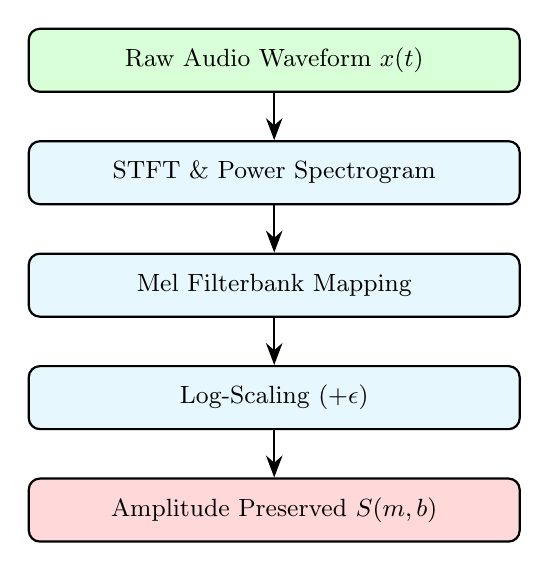
\begin{tikzpicture}[
    node distance=0.6cm,
    block/.style={rectangle, draw, thick, fill=cyan!10, text width=6cm, align=center, rounded corners, minimum height=0.8cm, font=\small},
    line/.style={draw, -{Stealth[scale=1.2]}, thick},
]
\node [block, fill=green!15] (input) {Raw Audio Waveform $x(t)$};
\node [block, below=of input] (stft) {STFT \& Power Spectrogram};
\node [block, below=of stft] (mel) {Mel Filterbank Mapping};
\node [block, below=of mel] (log) {Log-Scaling ($+ \epsilon$)};
\node [block, fill=red!15, below=of log] (output) {Amplitude Preserved $S(m,b)$};

\path [line] (input) -- (stft);
\path [line] (stft) -- (mel);
\path [line] (mel) -- (log);
\path [line] (log) -- (output);
\end{tikzpicture}
\caption{Acoustic Preprocessing Pipeline emphasizing amplitude preservation.}
\label{fig:preprocessing}
\end{figure}

\subsection{SE-ResNet Architecture}
The core processing engine is an attention-augmented Residual Network. The network ingests the 2D Mel-spectrogram and processes it through a series of residual blocks, each integrated with a Squeeze-and-Excitation (SE) module. Let $\mathbf{U} \in \mathbb{R}^{C \times H \times W}$ be the feature map output of a standard residual mapping. The SE block adaptively recalibrates channel-wise feature responses by explicitly modeling interdependencies between channels.

The \textit{Squeeze} operation aggregates spatial features via Global Average Pooling (GAP) to produce a channel descriptor $\mathbf{z} \in \mathbb{R}^{C}$:
\begin{equation}
    z_c = \frac{1}{H \times W} \sum_{i=1}^{H} \sum_{j=1}^{W} \mathbf{U}_{c}(i, j)
\end{equation}
The \textit{Excitation} operation employs a bottleneck architecture with two fully connected (FC) layers, regulated by a reduction ratio $r$, followed by a sigmoid activation to capture channel-wise dependencies:
\begin{equation}
    \mathbf{s} = \sigma\left( \mathbf{W}_2 \delta\left( \mathbf{W}_1 \mathbf{z} \right) \right)
\end{equation}
where $\delta$ is the ReLU activation, $\mathbf{W}_1 \in \mathbb{R}^{\frac{C}{r} \times C}$ and $\mathbf{W}_2 \in \mathbb{R}^{C \times \frac{C}{r}}$ are the trainable weights, and $\sigma$ is the sigmoid function. The final output is obtained by channel-wise multiplication: $\widetilde{\mathbf{U}}_c = s_c \cdot \mathbf{U}_c$. 
This dynamic recalibration ensures the network amplifies features critical to Doppler shift while suppressing invariant background noise.

\begin{figure*}[htbp]
\centering
\resizebox{\textwidth}{!}{
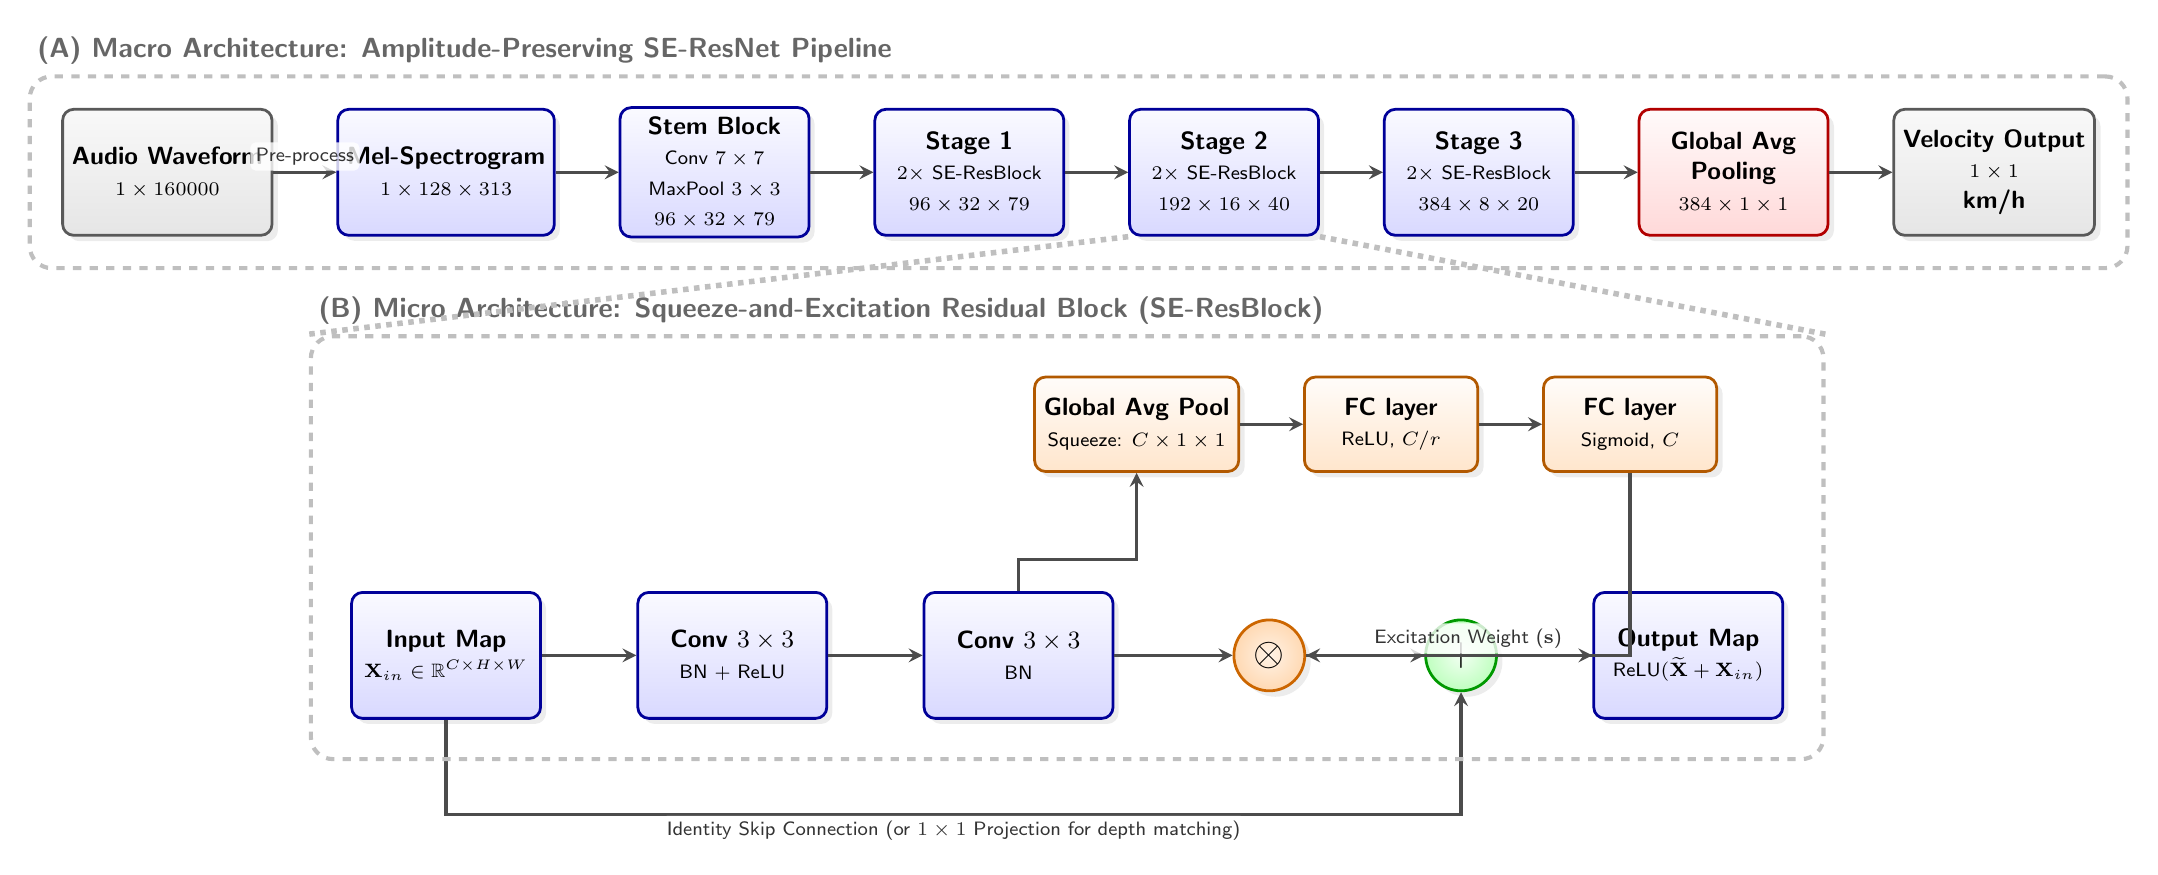
\begin{tikzpicture}[
    >=stealth,
    font=\sffamily\small,
    % Modern Gradient Styles
    tensor/.style={rectangle, draw=blue!60!black, line width=1pt, top color=blue!2, bottom color=blue!15, rounded corners=4pt, minimum width=2.4cm, minimum height=1.6cm, align=center, drop shadow={opacity=0.15, shadow xshift=2pt, shadow yshift=-2pt}},
    op/.style={circle, draw=green!60!black, line width=1pt, inner color=green!5, outer color=green!25, minimum size=0.9cm, align=center, drop shadow={opacity=0.15}, inner sep=0pt, font=\Large\bfseries},
    seop/.style={rectangle, draw=orange!70!black, line width=1pt, top color=orange!2, bottom color=orange!20, rounded corners=4pt, minimum width=2.2cm, minimum height=1.2cm, align=center, drop shadow={opacity=0.15}},
    gap/.style={rectangle, draw=red!70!black, line width=1pt, top color=red!2, bottom color=red!15, rounded corners=4pt, minimum width=2.4cm, minimum height=1.6cm, align=center, drop shadow={opacity=0.15}},
    io/.style={rectangle, draw=gray!70!black, line width=1pt, top color=gray!5, bottom color=gray!20, rounded corners=4pt, minimum width=2.4cm, minimum height=1.6cm, align=center, drop shadow={opacity=0.15}},
    arr/.style={->, line width=1.2pt, draw=black!70},
    dashedarr/.style={->, line width=1.2pt, dashed, draw=black!70},
    labelnode/.style={font=\sffamily\scriptsize\color{black!80}, align=center, fill=white, fill opacity=0.8, text opacity=1, rounded corners=2pt, inner sep=2pt}
]

% ========================================================
% PART 1: MACRO ARCHITECTURE (Top Row)
% ========================================================

\node[io] (audio) {\textbf{Audio Waveform}\\\scriptsize $1 \times 160000$};
\node[tensor, right=0.8cm of audio] (mel) {\textbf{Mel-Spectrogram}\\\scriptsize $1 \times 128 \times 313$};
\draw[arr] (audio) -- node[above, labelnode] {Pre-process} (mel);

\node[tensor, right=0.8cm of mel] (stem) {\textbf{Stem Block}\\\scriptsize Conv $7\times7$\\ \scriptsize MaxPool $3\times3$\\\scriptsize $96 \times 32 \times 79$};
\draw[arr] (mel) -- (stem);

\node[tensor, right=0.8cm of stem] (stage1) {\textbf{Stage 1}\\\scriptsize $2\times$ SE-ResBlock\\\scriptsize $96 \times 32 \times 79$};
\draw[arr] (stem) -- (stage1);

\node[tensor, right=0.8cm of stage1] (stage2) {\textbf{Stage 2}\\\scriptsize $2\times$ SE-ResBlock\\\scriptsize $192 \times 16 \times 40$};
\draw[arr] (stage1) -- (stage2);

\node[tensor, right=0.8cm of stage2] (stage3) {\textbf{Stage 3}\\\scriptsize $2\times$ SE-ResBlock\\\scriptsize $384 \times 8 \times 20$};
\draw[arr] (stage2) -- (stage3);

\node[gap, right=0.8cm of stage3] (gapnode) {\textbf{Global Avg}\\\textbf{Pooling}\\\scriptsize $384 \times 1 \times 1$};
\draw[arr] (stage3) -- (gapnode);

\node[io, right=0.8cm of gapnode] (output) {\textbf{Velocity Output}\\\scriptsize $1 \times 1$\\\textbf{km/h}};
\draw[arr] (gapnode) -- (output);

% Bounding Box for Macro
\node[draw=gray!50, line width=1.5pt, dashed, rounded corners=8pt, fit=(audio) (output), inner sep=0.4cm] (macrobox) {};
\node[anchor=south west, font=\sffamily\normalsize\bfseries, color=gray!80!black] at (macrobox.north west) {(A) Macro Architecture: Amplitude-Preserving SE-ResNet Pipeline};


% ========================================================
% PART 2: MICRO ARCHITECTURE (Bottom Row)
% ========================================================

\node[tensor, below=4.5cm of mel] (xin) {\textbf{Input Map}\\\scriptsize $\mathbf{X}_{in} \in \mathbb{R}^{C \times H \times W}$};

\node[tensor, right=1.2cm of xin] (conv1) {\textbf{Conv $3\times3$}\\\scriptsize BN + ReLU};
\draw[arr] (xin) -- (conv1);

\node[tensor, right=1.2cm of conv1] (conv2) {\textbf{Conv $3\times3$}\\\scriptsize BN};
\draw[arr] (conv1) -- (conv2);

% The Scale operation (Multiply) comes after Conv2, before Add
\node[op, inner color=orange!10, outer color=orange!30, draw=orange!80!black, right=1.5cm of conv2] (mult) {$\otimes$};
\draw[arr] (conv2) -- (mult);

\node[op, right=1.5cm of mult] (add) {$\mathbf{+}$};
\draw[arr] (mult) -- (add);

\node[tensor, right=1.2cm of add] (xout) {\textbf{Output Map}\\\scriptsize $\text{ReLU}(\widetilde{\mathbf{X}} + \mathbf{X}_{in})$};
\draw[arr] (add) -- (xout);

% Residual Skip Connection (Identity)
\draw[arr] (xin.south) -- ++(0, -1.2) -| node[pos=0.25, below, labelnode] {Identity Skip Connection (or $1\times1$ Projection for depth matching)} (add.south);

% SE Branch (Extracts from Conv2 output, injects into Multiplier)
\node[seop, above=1.5cm of conv2, xshift=1.5cm] (segap) {\textbf{Global Avg Pool}\\\scriptsize Squeeze: $C \times 1 \times 1$};
\draw[arr] (conv2.north) -- ++(0, 0.4) -| (segap.south);

\node[seop, right=0.8cm of segap] (fc1) {\textbf{FC layer}\\\scriptsize ReLU, $C/r$};
\draw[arr] (segap) -- (fc1);

\node[seop, right=0.8cm of fc1] (fc2) {\textbf{FC layer}\\\scriptsize Sigmoid, $C$};
\draw[arr] (fc1) -- (fc2);

\draw[arr] (fc2.south) |- node[pos=0.75, above, labelnode] {Excitation Weight ($\mathbf{s}$)} (mult.east);

% Bounding Box for Micro
\node[draw=gray!50, line width=1.5pt, dashed, rounded corners=8pt, fit=(xin) (xout) (segap) (fc2) (add), inner sep=0.5cm] (microbox) {};
\node[anchor=south west, font=\sffamily\normalsize\bfseries, color=gray!80!black] at (microbox.north west) {(B) Micro Architecture: Squeeze-and-Excitation Residual Block (SE-ResBlock)};

% Link Macro to Micro
\draw[gray!50, line width=2pt, dotted] (stage2.south west) -- (microbox.north west);
\draw[gray!50, line width=2pt, dotted] (stage2.south east) -- (microbox.north east);

\end{tikzpicture}
}
\caption{Detailed schematic of the Amplitude-Preserving SE-ResNet. \textbf{(A)} High-level macro architecture detailing the progression of tensor dimensions as the spatial resolution is downsampled and channel capacity is expanded. \textbf{(B)} Exploded micro-architecture of a single SE-ResBlock, illustrating the dual-path structure where the temporal/spatial features are processed by $3 \times 3$ convolutions, while the Squeeze-and-Excitation (SE) branch dynamically models cross-channel interdependencies to recalibrate the feature maps prior to the residual addition.}
\label{fig:architecture}
\end{figure*}

\subsection{Rigorous Evaluation Framework}
Due to the relatively small size of the VS13 dataset (400 samples), standard k-fold cross-validation is susceptible to optimism bias if hyperparameters are selected and evaluated on the same splits. To mitigate this, we implemented a \textit{Nested Cross-Validation} framework. Let $\mathcal{D}$ be the complete dataset. In the outer loop, $\mathcal{D}$ is partitioned into $K_{out} = 10$ folds. For each outer fold $k$, the test set $\mathcal{D}_{test}^{(k)}$ is isolated, and the remaining data $\mathcal{D}_{train}^{(k)}$ is passed to an inner optimization loop.

The performance metrics used are the Root Mean Square Error (RMSE) and Mean Absolute Error (MAE):
\begin{equation}
    \text{RMSE} = \sqrt{\frac{1}{N}\sum_{i=1}^{N}(y_i - \hat{y}_i)^2}
\end{equation}
\begin{equation}
    \text{MAE} = \frac{1}{N}\sum_{i=1}^{N}|y_i - \hat{y}_i|
\end{equation}
where $y_i$ and $\hat{y}_i$ are the true and predicted speeds for the $i$-th sample, and $N$ is the total number of samples evaluated.

\begin{figure}[htbp]
\centering
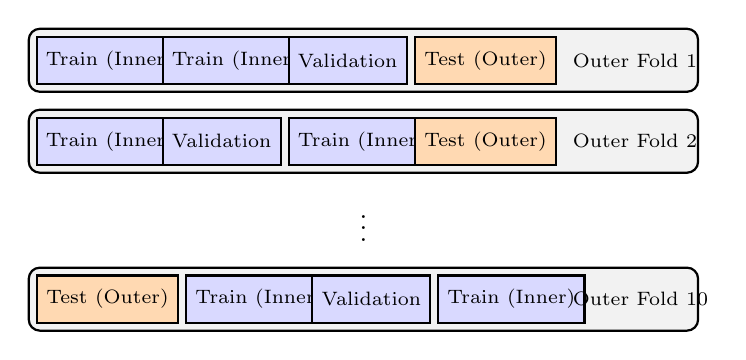
\begin{tikzpicture}[
    node distance=0.2cm,
    outer/.style={rectangle, draw, thick, rounded corners, minimum width=8.5cm, minimum height=0.8cm, fill=gray!10},
    inner/.style={rectangle, draw, thick, fill=blue!15, minimum width=1.5cm, minimum height=0.6cm, font=\scriptsize, anchor=west},
    test/.style={rectangle, draw, thick, fill=orange!30, minimum width=1.8cm, minimum height=0.6cm, font=\scriptsize, anchor=west}
]

% Fold 1
\node[outer] (fold1) {};
\node[inner] at ([xshift=0.1cm]fold1.west) {Train (Inner)};
\node[inner] at ([xshift=1.7cm]fold1.west) {Train (Inner)};
\node[inner] at ([xshift=3.3cm]fold1.west) {Validation};
\node[test]  at ([xshift=4.9cm]fold1.west) {Test (Outer)};
\node[anchor=west, font=\scriptsize] at ([xshift=6.8cm]fold1.west) {Outer Fold 1};

% Fold 2
\node[outer, below=of fold1] (fold2) {};
\node[inner] at ([xshift=0.1cm]fold2.west) {Train (Inner)};
\node[inner] at ([xshift=1.7cm]fold2.west) {Validation};
\node[inner] at ([xshift=3.3cm]fold2.west) {Train (Inner)};
\node[test]  at ([xshift=4.9cm]fold2.west) {Test (Outer)};
\node[anchor=west, font=\scriptsize] at ([xshift=6.8cm]fold2.west) {Outer Fold 2};

\node[below=0.2cm of fold2] (dots) {$\vdots$};

% Fold 10
\node[outer, below=0.2cm of dots] (foldk) {};
\node[test]  at ([xshift=0.1cm]foldk.west) {Test (Outer)};
\node[inner] at ([xshift=2.0cm]foldk.west) {Train (Inner)};
\node[inner] at ([xshift=3.6cm]foldk.west) {Validation};
\node[inner] at ([xshift=5.2cm]foldk.west) {Train (Inner)};
\node[anchor=west, font=\scriptsize] at ([xshift=6.8cm]foldk.west) {Outer Fold 10};

\end{tikzpicture}
\caption{Nested Cross-Validation protocol ensuring zero data leakage.}
\label{fig:nestedcv}
\end{figure}

\section{Experimental Setup}
The experimental pipeline was built using PyTorch and executed on a dual NVIDIA T4 GPU setup. To search the hyperparameter space efficiently, we employed the Tree-structured Parzen Estimator (TPE) algorithm via the Optuna \cite{ref11} framework. The optimization was decentralized using an SQLite backend to manage concurrency across both GPUs, preventing locking overhead. The search space included the learning rate, weight decay, SE reduction ratio ($r \in \{8, 16, 32\}$), and noise augmentation intensities. For ablation studies, deterministic seeds were enforced to ensure comparable initialization across different architectural variants.

\section{Results and Discussion}
\subsection{State-of-the-Art Evaluation}
The proposed model was evaluated against the 81 blind test samples. To ensure maximum robustness, we utilized a 10-Fold Ensemble strategy where predictions from 10 identical SE-ResNet models (trained on distinct stratified CV folds) were averaged. 

As shown in Table \ref{tab:sota}, the proposed Amplitude-Preserving SE-ResNet achieves a Root Mean Square Error (RMSE) of $5.41$~km/h and a Mean Absolute Error (MAE) of $4.19$~km/h. This not only significantly outperforms the previous baseline of $7.87$~km/h for single-modality acoustic methods \cite{ref9}, but it completely surpasses the multi-modal Audio-Visual state-of-the-art ($6.54$~km/h) \cite{ref10}, achieving a $1.13$~km/h absolute improvement while requiring only a single microphone.

To quantify the stability of the architecture, we also evaluated the expected performance of a \textit{single} model without ensembling. The average single-model performance across the 10 folds was $6.18 \pm 0.26$~km/h RMSE, confirming that even without the computational overhead of ensembling, the proposed architecture remains superior to existing methods. Furthermore, a One-Way ANOVA across the 13 vehicle classes yielded $F = 1.288$ ($p = 0.2458$), indicating that the model's accuracy is highly consistent regardless of vehicle type.

\begin{table}[htbp]
\centering
\caption{Comparison with State-of-the-Art on the VS13 Dataset}
\label{tab:sota}
\resizebox{\linewidth}{!}{
\begin{tabular}{lllc}
\hline
\textbf{Method} & \textbf{Modality} & \textbf{RMSE} & \textbf{MAE} \\
\hline
$\epsilon$-SVR (MA Features) \cite{ref13} & Audio & $6.92$ & - \\
1D-CNN (Raw Waveform) \cite{ref4} & Audio & $8.88$ & $5.96$ \\
$\epsilon$-SVR (Mel-Spectrogram) \cite{ref9} & Audio & $7.87$ & $6.02$ \\
Deep Wavelet-Fourier \cite{ref10} & Audio+Video & $6.54$ & $4.59$ \\
\hline
\textbf{Proposed SE-ResNet (Single)} & \textbf{Audio} & $6.18 \pm 0.26$ & $4.84 \pm 0.26$ \\
\textbf{Proposed SE-ResNet (10-Fold)} & \textbf{Audio} & $\mathbf{5.41}$ & $\mathbf{4.19}$ \\
\hline
\end{tabular}
}
\end{table}

\subsection{Systematic Ablation Study}
To isolate the contribution of individual architectural components and environmental augmentations, a rigorous ablation study was performed. Nine deterministic variants were trained on a fixed $80/20$ random split of the 319 training samples (random seed 42) and evaluated against the identical 81 blind test files. The results are summarized in Table \ref{tab:ablation}.

\begin{table}[htbp]
\centering
\caption{Systematic Ablation Study on Test Set (N=81)}
\label{tab:ablation}
\resizebox{\linewidth}{!}{
\begin{tabular}{llccc}
\hline
\textbf{Group} & \textbf{Variant} & \textbf{Params} & \textbf{RMSE} & \textbf{MAE} \\
\hline
\multicolumn{5}{l}{\textit{Squeeze-and-Excitation Ratio ($r$)}} \\
SE & Baseline (No SE) & 6.2M & 7.27 & 5.68 \\
SE & SE-ResNet (r=16)* & 6.3M & 6.55 & 5.19 \\
SE & SE-ResNet (r=8) & 6.3M & 6.39 & 5.15 \\
SE & SE-ResNet (r=32) & 6.2M & \textbf{5.78} & \textbf{4.47} \\
\hline
\multicolumn{5}{l}{\textit{Network Depth}} \\
Depth & Shallow (2 stages) & 1.5M & 9.10 & 7.41 \\
Depth & Standard (3 stages)* & 6.3M & 6.55 & 5.19 \\
Depth & Deep (4 stages) & 15.4M & \textbf{6.44} & \textbf{5.31} \\
\hline
\multicolumn{5}{l}{\textit{Acoustic Environment Augmentation}} \\
Aug & No Aug (Clean) & 6.3M & 6.39 & 4.84 \\
Aug & Standard Noise* & 6.3M & 6.55 & 5.19 \\
Aug & Heavy Noise & 6.3M & \textbf{6.15} & \textbf{4.69} \\
\hline
\multicolumn{5}{l}{\scriptsize *Denotes the Control Baseline configuration (r=16, 3 Stage, Std Noise).}
\end{tabular}
}
\end{table}

\textbf{Squeeze-and-Excitation:} The inclusion of SE blocks universally improved performance compared to the Baseline ResNet ($7.27$~km/h). Interestingly, on a single-fold basis, $r=32$ provided the strongest regularization ($5.78$~km/h), although $r=8$ was selected during global hyperparameter optimization. This highlights the importance of the SE mechanism in dynamically attending to relevant Doppler frequency bands while suppressing static noise.

\textbf{Network Depth:} The shallow 2-stage network severely underfitted the data ($9.10$~km/h), lacking the hierarchical receptive field necessary to capture complex velocity curves. Conversely, increasing depth to 4 stages yielded marginal improvements ($6.44$~km/h) over the 3-stage baseline ($6.55$~km/h) at the cost of more than doubling the parameter count (15.4M).

\textbf{Augmentation:} Surprisingly, Heavy Noise (SNR 0-10dB) resulted in the best single-model generalization ($6.15$~km/h) within this specific random fold, outperforming Clean Audio ($6.39$~km/h) and Standard Noise ($6.55$~km/h). This suggests that severe acoustic distortion forces the network to learn deeper, scale-invariant Doppler shift features rather than memorizing superficial amplitude patterns.

\subsection{Real-Time Deployment and Hardware Benchmarking}
To validate the model's suitability for real-world Intelligent Transportation Systems (ITS) deployment, we conducted rigorous hardware throughput and latency benchmarking. The evaluation isolated pure model inference speeds by executing forward passes on synthetically generated input tensors ($128 \times 313$ Mel-spectrograms), bypassing disk I/O bottlenecks. 

Experiments were performed on both an Edge CPU environment (simulating low-cost traffic cameras) and a cloud-tier NVIDIA T4 GPU using Automatic Mixed Precision (AMP). Furthermore, we evaluated the impact of PyTorch 2.0 Ahead-Of-Time (AOT) compilation, which utilizes OpenAI's Triton to mathematically fuse Conv2D, BatchNorm, and ReLU kernels.

\begin{table}[htbp]
\centering
\caption{Deployment Latency and Throughput Benchmarks}
\label{tab:benchmark}
\resizebox{\linewidth}{!}{
\begin{tabular}{lllccc}
\hline
\textbf{Device} & \textbf{Mode} & \textbf{Batch} & \textbf{Latency} & \textbf{P95} & \textbf{Samples/s} \\
\hline
\multicolumn{6}{l}{\textit{Edge CPU Environment (No AMP)}} \\
CPU & Single & 1 & 41.58 ms & 44.54 ms & 24.05 \\
CPU & 10-Fold & 1 & 414.25 ms & 437.81 ms & 2.41 \\
CPU & Single & 32 & 1227.67 ms & 1291.33 ms & 26.07 \\
\hline
\multicolumn{6}{l}{\textit{NVIDIA T4 GPU Environment (AMP Enabled)}} \\
CUDA & Single & 1 & 3.62 ms & 3.85 ms & 276.25 \\
CUDA & 10-Fold & 1 & 36.07 ms & 37.84 ms & 27.73 \\
CUDA & Single & 32 & 19.14 ms & 19.51 ms & 1671.82 \\
\hline
\multicolumn{6}{l}{\textit{NVIDIA T4 GPU with Kernel Fusion (Torch.Compile)}} \\
CUDA & Single & 1 & \textbf{2.28 ms} & \textbf{2.46 ms} & \textbf{439.19} \\
CUDA & Single & 32 & \textbf{14.61 ms} & \textbf{14.69 ms} & \textbf{2190.16} \\
\hline
\end{tabular}
}
\end{table}

As shown in Table \ref{tab:benchmark}, a single uncompiled SE-ResNet model achieves 24.05 samples per second on a pure CPU, confirming its viability for real-time edge processing (where audio is typically windowed at 1-2 Hz). 

On the T4 GPU, the standard PyTorch implementation achieves a maximum throughput of 1671.82 samples/s (Batch 32). However, by enabling AOT kernel fusion via \texttt{torch.compile}, latency dropped by $36\%$ (from 3.62~ms to 2.28~ms for real-time streaming) and bulk throughput skyrocketed to an exceptional 2,190.16 samples per second. Even the massive 10-Fold Ensemble is capable of running faster than real-time (27.73 samples/s) on the GPU. These results conclusively prove that the proposed architecture is not only highly accurate but also computationally lightweight enough for massive-scale deployment.

\section{Conclusion}

% To be written
\begin{thebibliography}{99}
\bibitem{ref1}
V. Cevher, R. Chellappa, and J. H. McClellan, "Vehicle speed estimation using acoustic wave patterns," \textit{IEEE Trans. Signal Process.}, vol. 57, no. 1, pp. 30-47, Jan. 2009.

\bibitem{ref2}
R. López-Valcarce, C. Mosquera, and F. Pérez-González, "Estimation of road vehicle speed using two omnidirectional microphones: A maximum likelihood approach," \textit{EURASIP J. Adv. Signal Process.}, vol. 2004, no. 8, 2004.

\bibitem{ref3}
H. Parineh, M. Sarvi, and S. A. Bagloee, "Acoustic Sensors and Audio Signal Processing in Intelligent Transportation Systems: A Survey," \textit{IEEE Transactions on Intelligent Vehicles}, 2024.

\bibitem{ref4}
I. Čavor and S. Djukanović, "Vehicle Speed Estimation From Audio Signals Using 1D Convolutional Neural Networks," in \textit{Proc. 27th Int. Conf. Inf. Technol. (IT)}, Feb. 2023, pp. 1-4.

\bibitem{ref5}
S. Djukanović, J. Matas, and T. Virtanen, "Acoustic Vehicle Speed Estimation from Single Sensor Measurements," \textit{IEEE Sensors Journal}, vol. 21, no. 20, pp. 23317-23324, Oct. 2021.

\bibitem{ref6}
S. Djukanović, N. Bulatović, and I. Čavor, "A dataset for audio-video based vehicle speed estimation," in \textit{Proc. 30th Telecommun. Forum (TELFOR)}, Nov. 2022, pp. 1-4.

\bibitem{ref7}
S. Djukanović, N. Bulatović, and I. Čavor, "A dataset for audio-video based vehicle speed estimation," \textit{arXiv preprint arXiv:2212.01651}, 2022.

\bibitem{ref8}
H. Parineh, M. Sarvi, and S. A. Bagloee, "MELAUDIS: A Large-Scale Benchmark Acoustic Dataset For Intelligent Transportation Systems Research," \textit{Scientific Data}, 2025.

\bibitem{ref13}
N. Bulatović and S. Djukanović, "An approach to improving sound-based vehicle speed estimation," in \textit{Proc. IEEE Zooming Innov. Consum. Technol. (ZINC)}, May 2022, pp. 108-112.

\bibitem{ref9}
N. Bulatović and S. Djukanović, "Mel-spectrogram features for acoustic vehicle-detection and speed estimation," in \textit{Proc. 26th Int. Conf. Inf. Technol. (IT)}, Feb. 2022, pp. 1-4.

\bibitem{ref10}
H. Parineh, M. Sarvi, and S. A. Bagloee, "A Deep Wavelet-Fourier Method for Monaural Vehicle Speed Estimation in Real-Life Settings," \textit{IEEE Sensors J.}, vol. 24, no. 9, pp. 15337-15346, May 2024.

\bibitem{ref11}
T. Akiba, S. Sano, T. Yanase, T. Ohta, and M. Koyama, "Optuna: A next-generation hyperparameter optimization framework," in \textit{Proc. 25th ACM SIGKDD Int. Conf. Knowl. Discovery Data Mining (KDD)}, 2019, pp. 2623-2631.

\bibitem{ref12}
J. Hu, L. Shen, and G. Sun, "Squeeze-and-Excitation Networks," in \textit{Proc. IEEE Conf. Comput. Vis. Pattern Recognit. (CVPR)}, 2018, pp. 7132-7141.

\end{thebibliography}

\end{document}
